\chapter{Physically-Inspired Excitations}\label{ch:physInspExcitations}
This short chapter introduces several simple ways to excite the different resonators presented in Part \ref{part:resonators}.

\section{Initial conditions}
The easiest way to excite a system is to set its initial conditions to non-zero values. This has been done several times before using a raised cosine 

To not give the system an initial velocity, both $u^0$ and $u^1$ will have to be initialised with the same value

\subsection{Impulse}
The simplest way of exciting a system is to add an impulse to 

spatial Nyquist

\def\figWidth{0.32}
\begin{figure}[h]
    \centering
    \subfloat[$n = 1$.\label{fig:impulse1}]{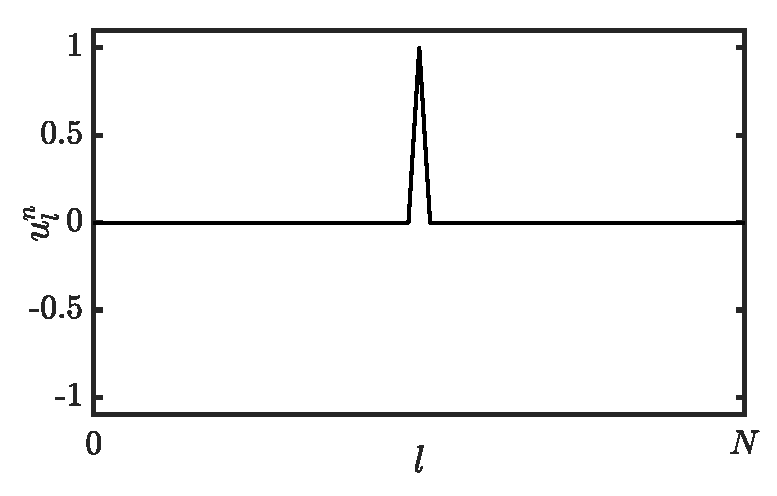
\includegraphics[width=\figWidth\textwidth]{figures/exciters/physInsp/impulse1.eps}}\hfill
    \subfloat[$n = 5$.\label{fig:impulse2}]{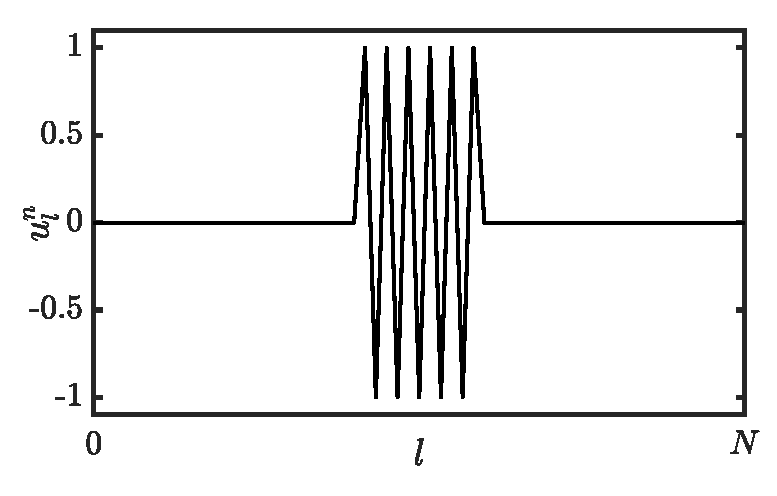
\includegraphics[width=\figWidth\textwidth]{figures/exciters/physInsp/impulse2.eps}}\hfill
    \subfloat[$n = 9$.\label{fig:impulse3}]{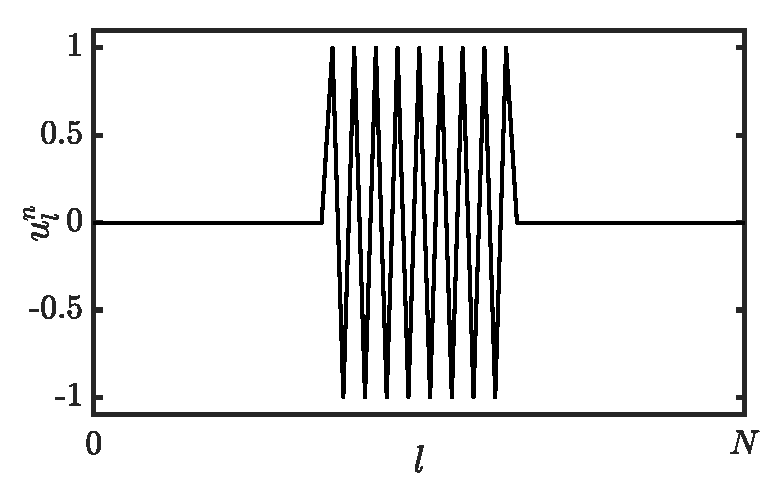
\includegraphics[width=\figWidth\textwidth]{figures/exciters/physInsp/impulse3.eps}}
    \caption{The 1D wave equation initialised with an impulse at $l=0.5N$.\label{fig:impulse}}
\end{figure}

\subsection{Raised cosine}\label{sec:raisedCosine}
As the impulse triggers very high-frequency behaviour 

Also referred to as a pluck -- due to the displacing and letting go -- but a more physically reasonable pluck is presented in Section \ref{sec:pluck}

Simplest way is \texttt{hann}.

\def\figWidth{0.32}
\begin{figure}[h]
    \centering
    \subfloat[$n = 1$.\label{fig:raisedCos1}]{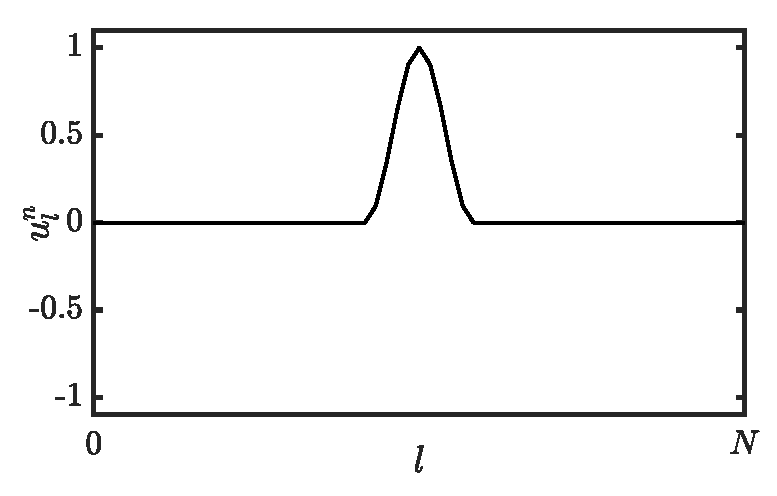
\includegraphics[width=\figWidth\textwidth]{figures/exciters/physInsp/raisedCos1.eps}}\hfill
    \subfloat[$n = 5$.\label{fig:raisedCos2}]{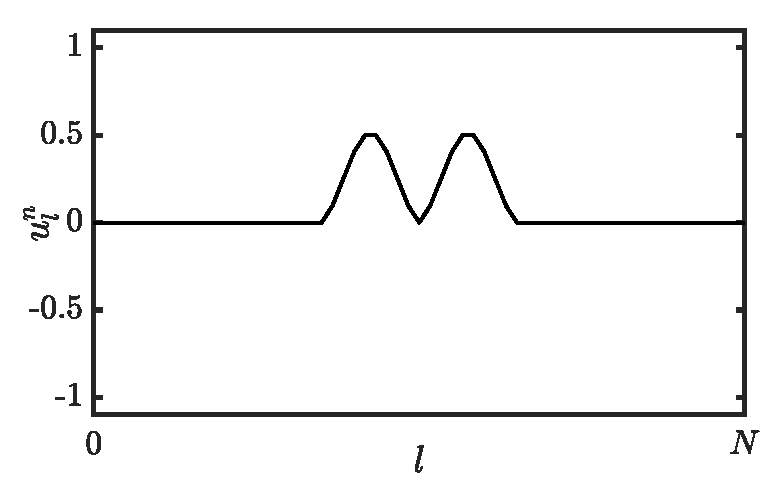
\includegraphics[width=\figWidth\textwidth]{figures/exciters/physInsp/raisedCos2.eps}}\hfill
    \subfloat[$n = 9$.\label{fig:raisedCos3}]{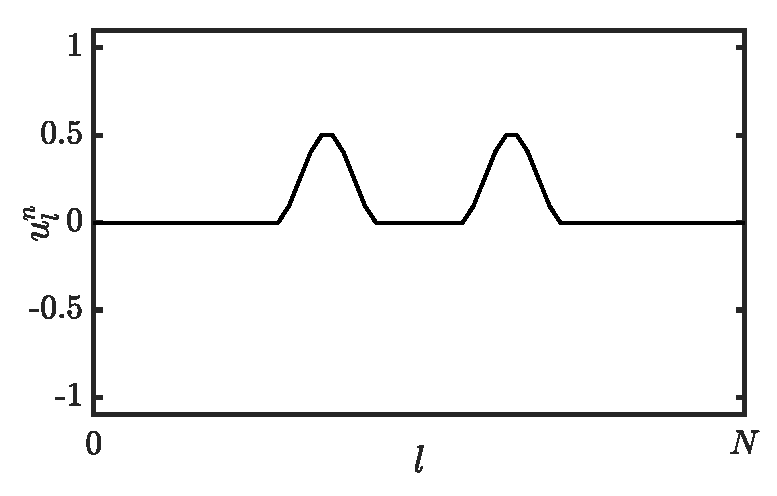
\includegraphics[width=\figWidth\textwidth]{figures/exciters/physInsp/raisedCos3.eps}}
    \caption{The 1D wave equation initialised with a raised cosine at $l=0.5N$.\label{fig:raisedCos}}
\end{figure}

\subsubsection{Strike}\label{sec:strike}
If $u^0_l$ is not set to be the same value as $u_l^1$ at the start of the simulation, one can model a strike. 

As can be observed from Figure \ref{fig:strike}, the amplitude of the displacement will be higher and, in the case of the 1D wave equation excited with a raised cosine, can be calculated to have a maximum amplitude of half the sum of the excitation. 


\def\figWidth{0.32}
\begin{figure}[h]
    \centering
    \subfloat[$n = 1$.\label{fig:strike1}]{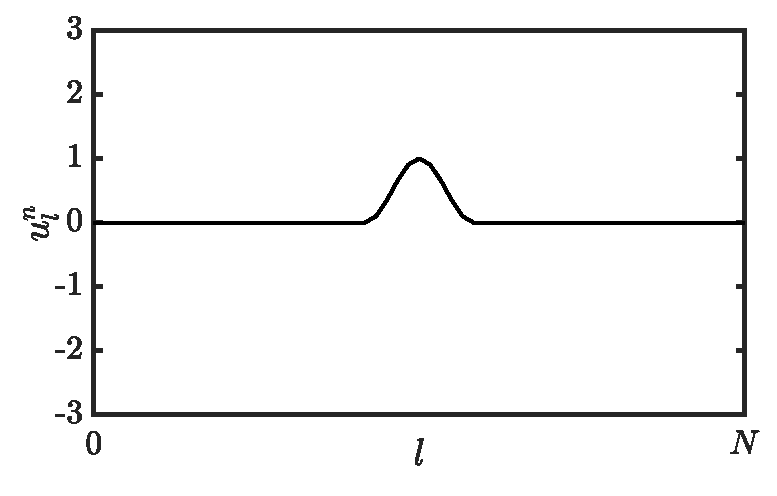
\includegraphics[width=\figWidth\textwidth]{figures/exciters/physInsp/strike1.eps}}\hfill
    \subfloat[$n = 5$.\label{fig:strike2}]{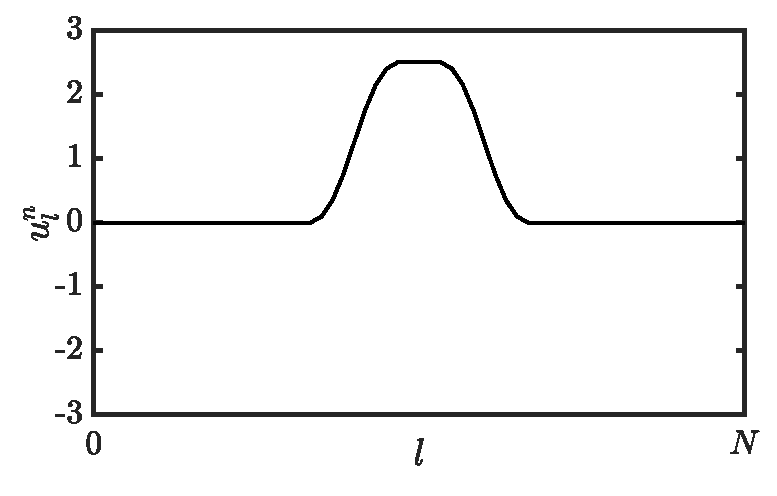
\includegraphics[width=\figWidth\textwidth]{figures/exciters/physInsp/strike2.eps}}\hfill
    \subfloat[$n = 9$.\label{fig:strike3}]{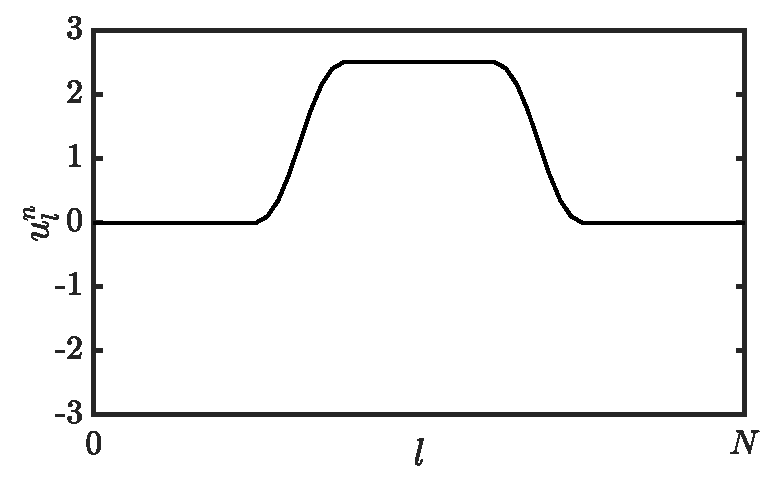
\includegraphics[width=\figWidth\textwidth]{figures/exciters/physInsp/strike3.eps}}
    \caption{The 1D wave equation initialised with a strike at $l=0.5N$. Notice the scaling of the y-axis compared to the other figures. \label{fig:strike}}
\end{figure}

\subsection{Pluck}\label{sec:pluck}
\begin{itemize}
    \item Cut-off raised cosine
    \item Triangle (for string)
\end{itemize}

\subsection{Noise}
Noise input

Stress-testing

\section{Time-varying excitations}
If one would like to excite the system, not at the start, but later on in the simulation, 

\begin{equation}
    \dtt \uln = c^2 \dxx \uln + F(t)
\end{equation}
where $F$ is a scaled force with units of m/s
if $c=\sqrt{T/\rho A}$, then $F = f/\rho A$, $f$ being a force in Newtons.


\subsection{Alternative pluck}
SMC figure

\subsection{Hammer}


\subsection{Pulse train}
For brass


